This chapter documents how KickSense was built, in the order the data actually flows through it. It begins with the system architecture and the constraints that shaped it, then follows a single penalty clip from an uncut source video through frame extraction, pose estimation, normalisation, resampling and tensor construction, into the model, through the loss function and the training procedure, and finally out through evaluation and the demonstration interface. Every constant quoted in this chapter is the value present in the corresponding source file, and every stage writes its output to disk so that the numbers reported in Chapter 4 can be regenerated without repeating earlier work.

\section{System Architecture}

KickSense is organised into four layers with strictly one directional data dependencies, so that any layer can be replaced without disturbing the layers beneath it.

The data layer owns everything on disk. It contains the source videos under \texttt{data/videos}, the extracted frames under \texttt{data/frames}, the landmark arrays under \texttt{data/keypoints}, the model ready tensors and split indices under \texttt{data/processed}, the single annotation spreadsheet at \texttt{data/labels/penalty\_labels.xlsx} which acts as the authoritative label source, and the trained checkpoints and evaluation artefacts under \texttt{outputs}.

The processing layer contains the computational stages. It runs frame extraction, MediaPipe pose estimation, the normalisation and resampling logic, model construction and training, and inference. It reads from and writes to the data layer and has no knowledge of any interface.

The service layer wraps inference behind a FastAPI application that accepts a video file, executes the same preprocessing path used during training, and returns a JSON document containing the predicted direction, the full softmax distribution over the three classes, and the predicted power. This layer exists specifically so that the mobile client planned in Chapter 5 does not need to reimplement any preprocessing.

The presentation layer is the Streamlit application, which accepts an uploaded clip, renders the pose overlay so that a user can see exactly what the model observed, and displays the prediction alongside its confidence distribution.

\begin{figure}[H]
    \centering
    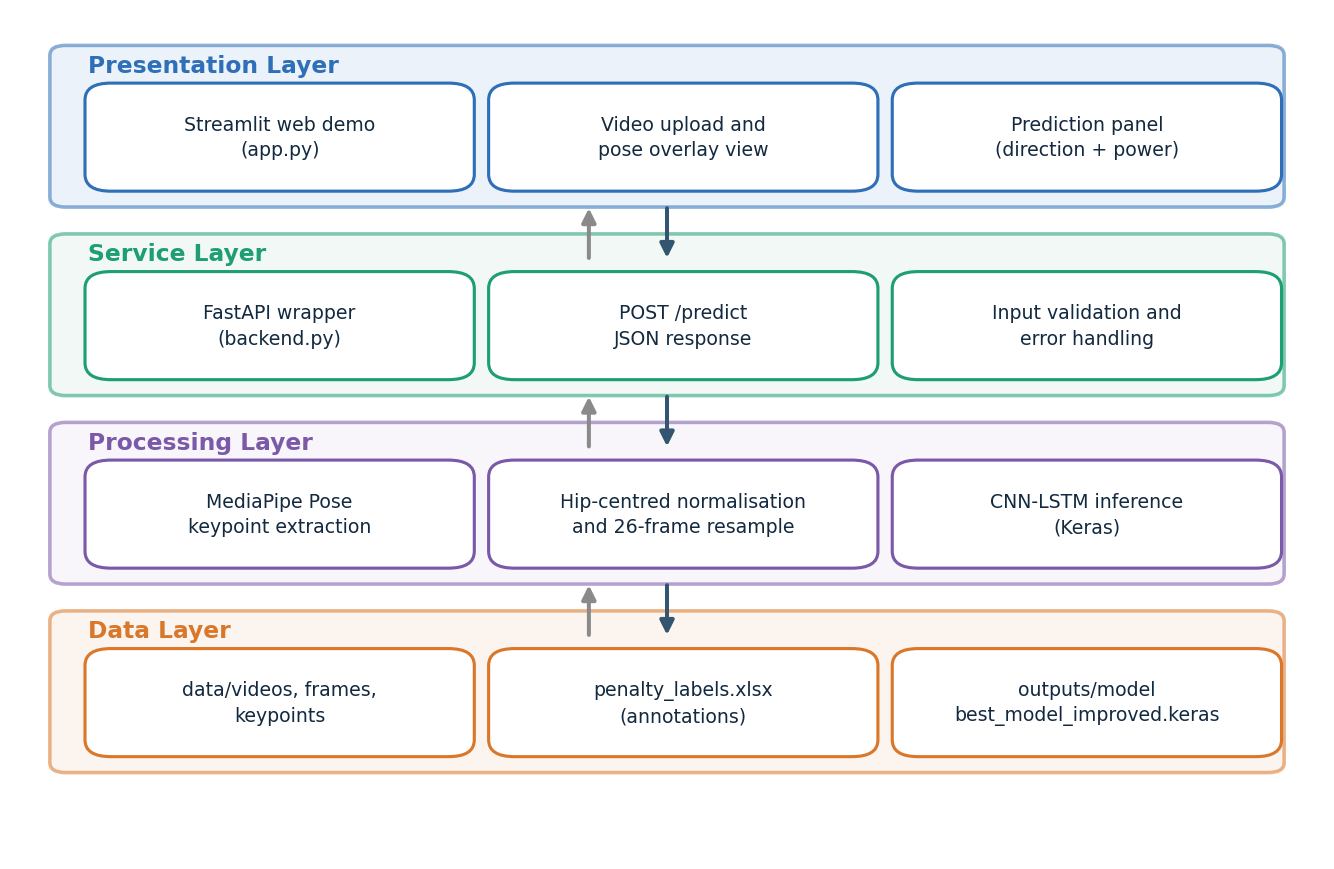
\includegraphics[width=0.99\textwidth]{fig04_system_architecture.png}
    \caption{Layered system architecture of KickSense}
    \label{fig:architecture}
\end{figure}

\noindent
\textbf{Description:} This diagram shows the four layers and the direction of their dependencies. Downward arrows indicate calls into the layer below and upward arrows indicate returned results. The presentation and service layers both route through the identical processing layer code path, which is the mechanism that prevents the preprocessing of an uploaded clip from drifting away from the preprocessing applied during training.

\section{Design Constraints}

\begin{itemize}
    \item \textbf{Hardware constraint:} the entire pipeline, including training, must run on a consumer laptop without a dedicated graphics processor. This single constraint rules out three dimensional convolution over pixel volumes and rules out the heavier pose estimators, and it is the reason the model is limited to roughly a quarter of a million parameters.
    \item \textbf{Input constraint:} the system must accept ordinary single camera video with no calibration, no known camera position and no depth sensor. Any representation that depends on knowing where the camera is cannot be used.
    \item \textbf{Data constraint:} no public dataset supervises this task, so the amount of labelled data is bounded by what could be manually annotated within the project timeline. Two hundred and twenty five usable sequences is the working figure, and every architectural decision was taken with that number in mind.
    \item \textbf{Software environment:} Python 3.12 inside a dedicated virtual environment named \texttt{kicksense\_env}, with TensorFlow and Keras for modelling, MediaPipe for pose estimation, OpenCV for video decoding, scikit-learn for splitting and metrics, pandas and openpyxl for the annotation file, and matplotlib for figure generation.
    \item \textbf{Reproducibility constraint:} all random seeds are fixed, the train, validation and test split is deterministic given a fixed random state, and all intermediate artefacts persist on disk, so that any reported number can be regenerated.
    \item \textbf{Honesty constraint:} the system must report its own failure rate rather than silently degrading. This is why the pose quality gate exists and why its rejection count is reported in Chapter 4 rather than omitted.
\end{itemize}

\section{Design Methodology}

The project follows an incremental, artefact driven methodology in which each stage is completed and persisted before the next begins. The reasoning is that the expensive and irreversible work in this project is data collection and annotation, not modelling, so the pipeline was deliberately built so that modelling experiments are cheap and repeatable while data work is done once.

\begin{itemize}
    \item \textbf{Partitioning:} the pipeline is decomposed into single responsibility scripts, namely frame extraction, pose estimation, preprocessing, training, and evaluation. Each is executable independently and each consumes only files written by an earlier stage.
    \item \textbf{Shared constants:} preprocessing constants such as the sequence length, the minimum detected frame count and the minimum detection ratio are declared once and imported wherever they are needed, which prevents the training and inference paths from diverging.
    \item \textbf{Deterministic splitting:} the train, validation and test partition is produced by a stratified split with a fixed random state, so the same clips land in the same partition on every run and results across experiments remain comparable.
    \item \textbf{Ablation by substitution:} because the architecture is constructed by a single builder function parameterised by variant, augmentation and regularisation flags, an ablation configuration differs from the full model by exactly one argument, which is what makes the attribution in Chapter 4 valid.
\end{itemize}

\section{High Level Design of the Pipeline}

\begin{figure}[H]
    \centering
    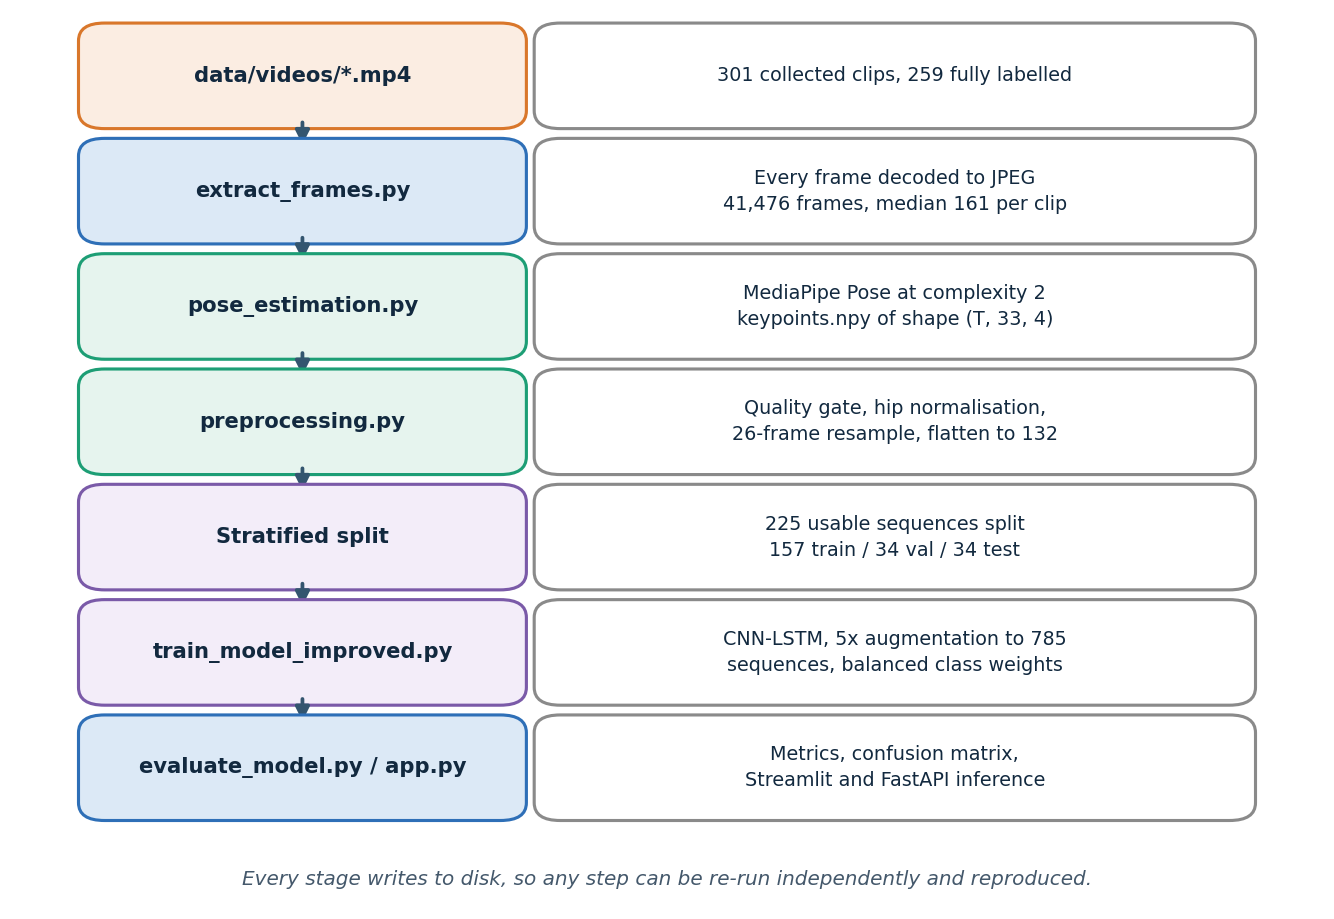
\includegraphics[width=0.92\textwidth]{fig05_pipeline_flow.png}
    \caption{End to end data pipeline from raw video to prediction}
    \label{fig:pipeline}
\end{figure}

\noindent
\textbf{Description:} This diagram traces the complete pipeline. The left column names the script or stage and the right column states what that stage produces, including the concrete quantities involved: three hundred and one collected clips reduced to two hundred and fifty nine annotated clips, variable length frame sequences reduced to a fixed twenty six step tensor, two hundred and twenty five usable sequences split into one hundred and fifty seven training, thirty four validation and thirty four test examples, and one hundred and fifty seven training sequences expanded to seven hundred and eighty five by fivefold augmentation.

\subsection{Stage One: Clip Preparation}

Source footage arrives in two forms. Broadcast material was obtained for penalties from a range of competitions and cut down so that each resulting file contains a single penalty, beginning shortly before the run up and ending shortly after contact. Locally recorded material was captured specifically for this project to increase the volume of the corpus and, more importantly, to add camera angles and framing that broadcast footage does not provide. The cutting was performed by a family of small scripts, each handling one source match, and the result is three hundred and one video files under \texttt{data/videos}.

\subsection{Stage Two: Frame Extraction}

Each video is decoded with OpenCV and every frame is written to disk as a JPEG image inside a per clip directory under \texttt{data/frames}. No subsampling is applied at this stage, deliberately, because discarding frames before pose estimation would discard information that the temporal resampling step is better placed to discard later, and because retaining all frames makes the detection ratio a meaningful diagnostic. Across the corpus this yields a mean of one hundred and sixty one frames per clip with a median of one hundred and sixty one, and the distribution together with the frame budget actually consumed is reported in Chapter 4.

\subsection{Stage Three: Pose Estimation}

Every extracted frame is passed through MediaPipe Pose. The configuration used is \texttt{static\_image\_mode=True}, \texttt{model\_complexity=2} and \texttt{min\_detection\_confidence=0.5}. The highest model complexity is chosen because accuracy of the landmark positions matters more than throughput in an offline batch stage. For each frame in which a pose is detected, the thirty three landmarks are recorded, each as four values, namely the horizontal coordinate normalised to the image width, the vertical coordinate normalised to the image height, a depth estimate relative to the hip midpoint, and a visibility confidence. Frames in which no pose is detected contribute nothing. The per clip result is an array of shape number of detected frames by thirty three by four, saved as \texttt{keypoints.npy} inside the clip directory under \texttt{data/keypoints}.

\begin{figure}[H]
    \centering
    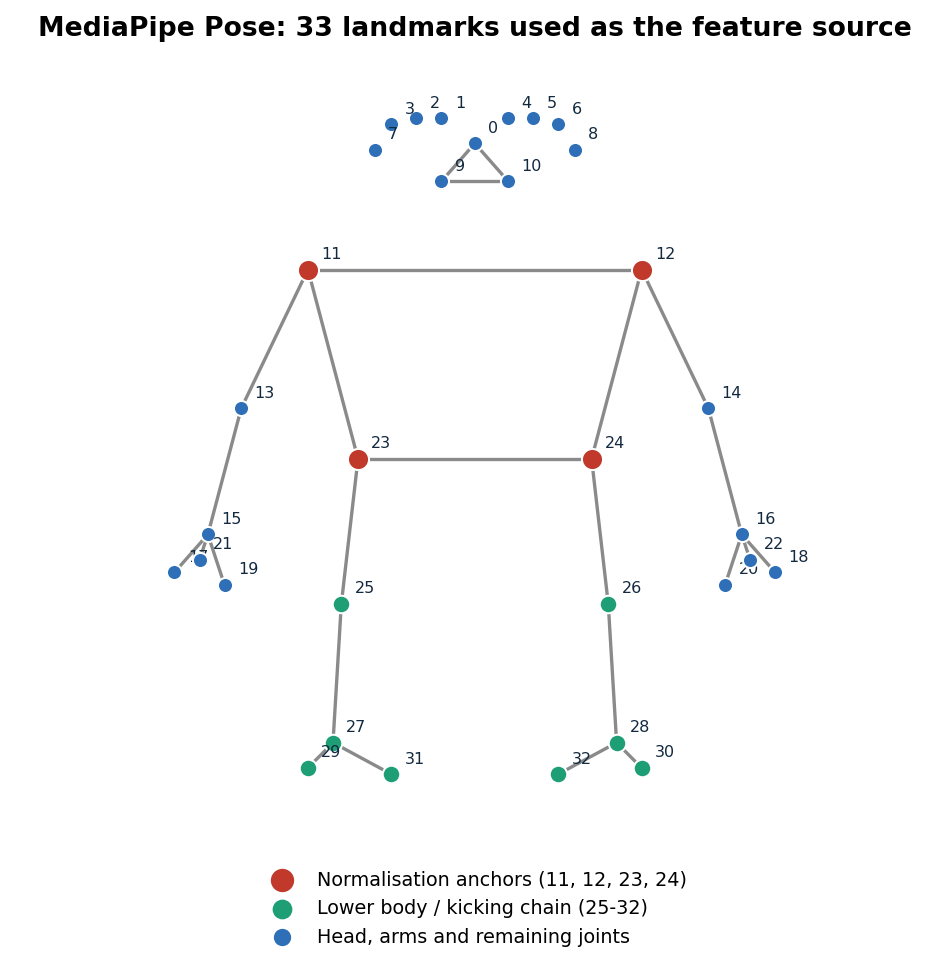
\includegraphics[width=0.72\textwidth]{fig07_mediapipe_landmarks.png}
    \caption{The 33 MediaPipe Pose landmarks and their role in KickSense}
    \label{fig:landmarks}
\end{figure}

\noindent
\textbf{Description:} This figure shows the landmark topology that defines the feature space. Landmarks eleven and twelve are the shoulders and landmarks twenty three and twenty four are the hips; these four are highlighted in red because they are used as the anchors for normalisation rather than merely as features. The lower body chain from landmark twenty five to landmark thirty two, highlighted in green, carries the kicking motion and is the region that both the perceptual literature and the base paper identify as most influential. The remaining landmarks are retained as features without playing a structural role.

\subsection{Stage Four: Preprocessing and Normalisation}

This stage converts variable length, camera dependent landmark streams into fixed size, camera independent tensors. It is the most consequential stage in the pipeline and proceeds in seven steps.

\begin{figure}[H]
    \centering
    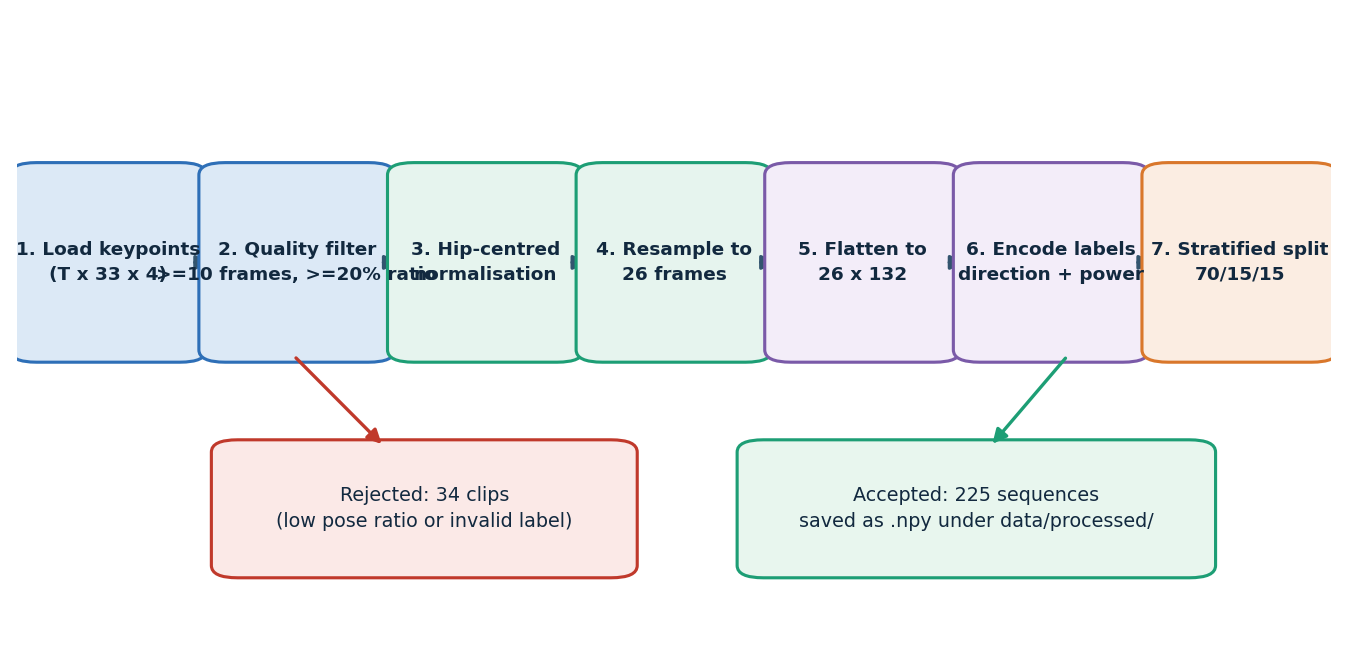
\includegraphics[width=0.99\textwidth]{fig08_preprocessing_flow.png}
    \caption{Preprocessing activity flow with the quality gate outcome}
    \label{fig:preprocessing}
\end{figure}

\noindent
\textbf{Description:} This activity diagram shows the seven preprocessing steps and, critically, the two possible outcomes of the quality gate. Clips that pass are written to \texttt{data/processed} as model ready sequences, and clips that fail are rejected and excluded from all subsequent stages, which is what converts a hidden pose estimation failure into a counted and reported quantity.

\begin{enumerate}[label=\arabic*.]
    \item \textbf{Load the landmark array.} The saved array of shape number of detected frames by thirty three by four is read from disk together with the total number of extracted frames for that clip, which is needed to compute the detection ratio.

    \item \textbf{Apply the quality gate.} A clip is rejected if it contains fewer than \texttt{MIN\_DETECTED\_FRAMES}, set to ten, or if the ratio of detected frames to extracted frames falls below \texttt{MIN\_POSE\_RATIO}, set to 0.20. The absolute threshold guards against clips too short to resample meaningfully, and the ratio threshold guards against clips in which MediaPipe succeeded only sporadically, since such clips produce a skeleton stream with large temporal gaps that resampling would paper over by interpolating across genuinely unobserved motion.

    \item \textbf{Normalise for camera position and player scale.} For each frame independently, the midpoint of the two hip landmarks, twenty three and twenty four, is computed and subtracted from every landmark, which places the origin at the player's pelvis and removes any dependence on where in the frame the player stands. A torso height is then computed as the vertical distance between the shoulder midpoint, from landmarks eleven and twelve, and the hip midpoint, and every coordinate is divided by that length, which removes the apparent size of the player and therefore the distance from the camera. What survives this operation is the shape of the body and how that shape changes over time, expressed in units of the player's own torso.

    \item \textbf{Resample to a fixed length.} Clips have different durations and different frame rates, so the detected frame sequence is resampled to exactly \texttt{SEQUENCE\_LENGTH}, set to twenty six, time steps by linear index interpolation. Sequences longer than twenty six frames are subsampled across their whole duration rather than truncated, so the run up, the plant and the strike are all represented; sequences shorter than twenty six frames are interpolated up. The value twenty six is a compromise between retaining enough temporal detail to distinguish the phases of the kick and keeping the input small enough that a quarter million parameter model is not immediately overparameterised.

    \item \textbf{Flatten to a feature vector.} The thirty three landmarks by four values per time step are flattened into a single vector of one hundred and thirty two features, producing a per clip tensor of shape twenty six by one hundred and thirty two. This is the exact input the model consumes.

    \item \textbf{Encode the labels.} The shot direction string is mapped to an integer, with left encoded as zero, centre as one and right as two, and is one hot encoded for the classification head. The shot power label is divided by ten so that it occupies the unit interval, which matches the sigmoid activation of the regression head, and predictions are multiplied by ten again at inference so that the reported value is on the original one to ten scale.

    \item \textbf{Split the dataset.} A stratified split with a fixed random state of forty two holds out fifteen percent as the test set, then splits the remainder with a proportion of 0.176 to produce the validation set, giving final sizes of one hundred and fifty seven training, thirty four validation and thirty four test sequences with the class proportions preserved in every partition.
\end{enumerate}

\subsection{Frames Extracted Against Frames Used}

The distinction between frames extracted and frames used matters and is easy to state precisely. Every frame of every clip is extracted and every extracted frame is submitted to MediaPipe, so pose estimation runs on the full corpus. The model, however, consumes exactly twenty six time steps per clip, so the temporal resampling step reduces a clip of one hundred and sixty one detected frames to twenty six representative steps. Averaged over the corpus this means roughly one sixth of the extracted frames contribute directly to a model input, with the remainder contributing indirectly by determining which frames the resampling selects and by establishing the detection ratio that the quality gate depends on. The exact totals across the whole corpus are reported in Chapter 4.

\begin{figure}[H]
    \centering
    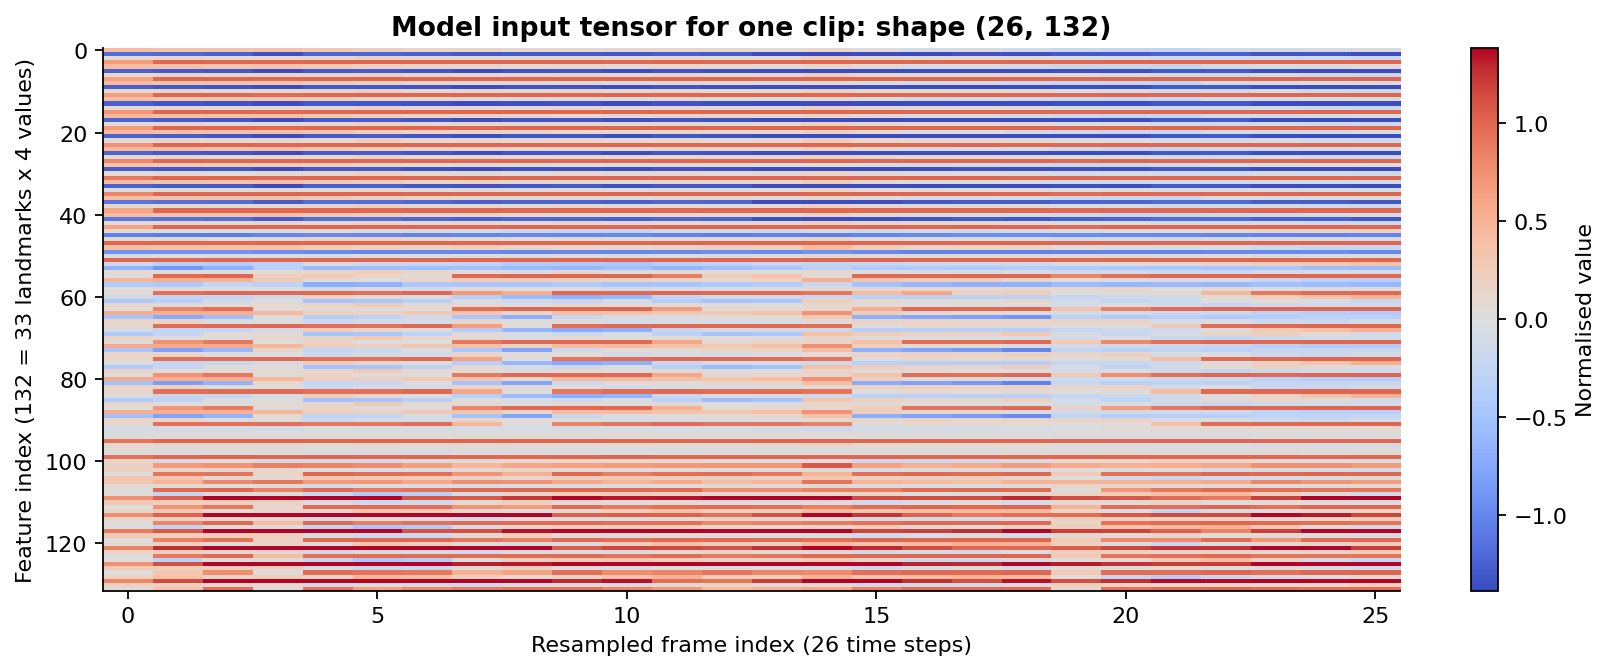
\includegraphics[width=0.99\textwidth]{fig27_feature_tensor.png}
    \caption{The model input tensor for a single clip, of shape 26 by 132}
    \label{fig:feature-tensor}
\end{figure}

\noindent
\textbf{Description:} This heatmap visualises one complete model input. The horizontal axis is the twenty six resampled time steps and the vertical axis is the one hundred and thirty two features, ordered as thirty three landmarks each contributing a horizontal coordinate, a vertical coordinate, a depth value and a visibility score. The horizontal banding shows that individual landmarks maintain a stable value across the sequence while specific rows, corresponding to the limbs involved in the kick, vary strongly over time. This variation is the signal the convolutional and recurrent layers are designed to detect.

\begin{figure}[H]
    \centering
    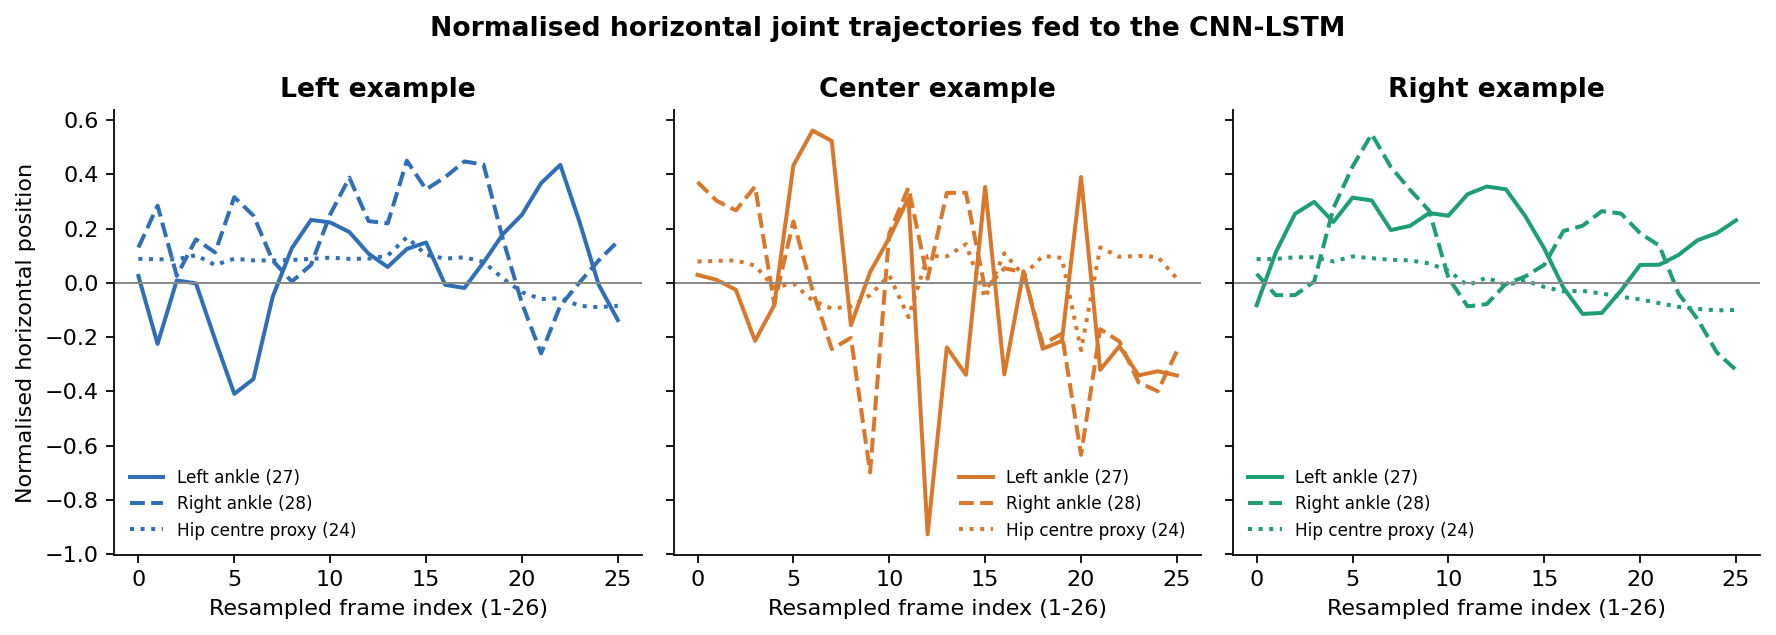
\includegraphics[width=0.99\textwidth]{fig26_pose_trajectories.png}
    \caption{Normalised horizontal joint trajectories for one example from each direction class}
    \label{fig:trajectories}
\end{figure}

\noindent
\textbf{Description:} This figure plots the normalised horizontal position of the two ankle landmarks and one hip landmark across the twenty six time steps, for one training example from each of the three direction classes. It demonstrates two things. First, the normalisation is working, because the trajectories are centred near zero and expressed on a comparable scale despite the source clips being filmed differently. Second, the classes are not trivially separable, since the trajectories overlap substantially, which is consistent with the moderate accuracy reported in Chapter 4 and explains why a temporal model rather than a simple threshold on a single landmark is required.

\section{Low Level Design of the Model}

\subsection{Architecture}

The model is a multi task network with a shared encoder and two task specific heads. The encoder combines one dimensional convolution with stacked recurrence, which reflects a specific hypothesis about the data. The convolutional front end operates across the time axis with a kernel of width three, so each filter observes three consecutive time steps and learns short range local motion primitives such as the acceleration of a limb or a change in the direction of a joint's travel. The recurrent back end then integrates these primitives over the full sequence, which is what allows the model to represent the ordering of the phases of the kick rather than merely their presence.

\begin{figure}[H]
    \centering
    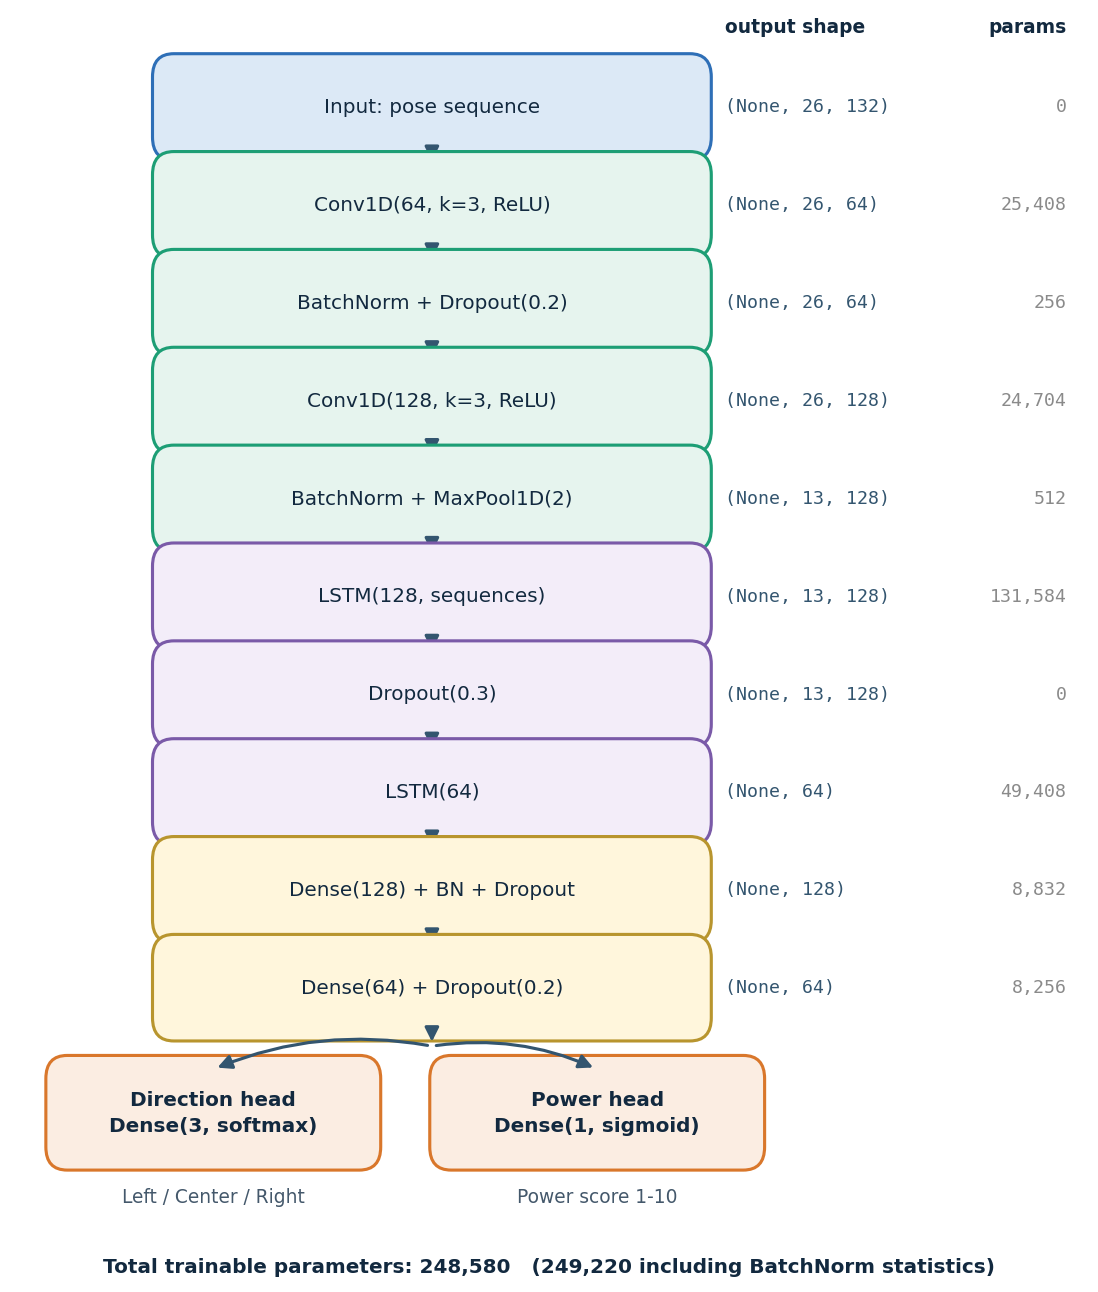
\includegraphics[width=0.80\textwidth]{fig06_model_architecture.png}
    \caption{Layer by layer architecture of the multi-task CNN-LSTM with tensor shapes and parameter counts}
    \label{fig:model}
\end{figure}

\noindent
\textbf{Description:} This diagram gives the complete architecture with the output shape and parameter count of every layer. The input of twenty six by one hundred and thirty two passes through two convolutional blocks that expand the channel dimension from one hundred and thirty two to sixty four and then to one hundred and twenty eight while max pooling halves the temporal dimension from twenty six to thirteen. Two stacked recurrent layers reduce the sequence to a single sixty four dimensional vector, two dense layers refine it, and the representation then branches into a three way softmax head for direction and a single unit sigmoid head for power. The total is 249,220 parameters of which 248,580 are trainable, the remaining 640 being the non trainable running statistics of the batch normalisation layers.

The two heads share the entire encoder, which is the central design decision of the model. The reasoning is sample efficiency. The body motion that determines where the ball is going is the same motion that determines how hard it will be struck, so training two separate networks on two hundred and twenty five sequences would learn the same representation twice from half as much effective supervision. Sharing the encoder means the direction labels also contribute gradient signal to the features the power head uses, and vice versa.

\subsection{Loss Function}

Training minimises a weighted sum of two losses computed on the two heads:
\[
\mathcal{L} = \lambda_{d}\,\mathcal{L}_{\text{CE}}(y_{d}, \hat{y}_{d}) \;+\; \lambda_{p}\,\mathcal{L}_{\text{MSE}}(y_{p}, \hat{y}_{p})
\]
where the direction term is the categorical cross entropy over the three classes,
\[
\mathcal{L}_{\text{CE}}(y_{d}, \hat{y}_{d}) = -\sum_{c=1}^{3} y_{d,c}\log \hat{y}_{d,c}
\]
and the power term is the mean squared error on the unit interval,
\[
\mathcal{L}_{\text{MSE}}(y_{p}, \hat{y}_{p}) = \frac{1}{N}\sum_{i=1}^{N}\left(\frac{p_{i}}{10} - \hat{p}_{i}\right)^{2}.
\]
The weights are set to $\lambda_{d} = 1.0$ and $\lambda_{p} = 0.3$. The asymmetry is deliberate and follows directly from the data. Direction is objectively verifiable from the footage and is the primary deliverable, whereas the power label is a subjective human judgement on a coarse ordinal scale and therefore carries substantial noise. Weighting the power term at three tenths allows it to shape the shared representation without allowing a noisy target to dominate the gradient and degrade the classification the system is primarily judged on.

\subsection{Class Weighting}

Balanced class weights are computed from the augmented training labels using the standard inverse frequency formulation, in which the weight of class $c$ is
\[
w_{c} = \frac{N}{K \cdot n_{c}}
\]
with $N$ the total number of training samples, $K$ the number of classes and $n_{c}$ the count of class $c$. One implementation detail is worth recording because it materially affects the interpretation of results. Keras does not accept a \texttt{class\_weight} argument for a model with more than one output, so the production training script computes these weights but does not in fact apply them during fitting. For the controlled experiments reported in Chapter 4 the weights are instead applied as per sample weights attached to the direction head, which is the functionally equivalent mechanism that Keras does support for multi output models. This is why the ablation table contains an explicit row with and without class weighting, and why the configuration matching the production script is the one labelled as omitting them.

\subsection{Data Augmentation}

The one hundred and fifty seven training sequences are expanded fivefold to seven hundred and eighty five by generating four additional variants of every sequence. Augmentation is applied to the training partition only; the validation and test partitions remain untouched.

\begin{itemize}
    \item \textbf{Gaussian noise.} Zero mean noise with a standard deviation of 0.01 is added to every coordinate, which models the jitter that a pose estimator produces on real footage and discourages the model from depending on landmark positions to a precision the estimator does not deliver.
    \item \textbf{Uniform scaling.} The whole sequence is multiplied by a factor drawn uniformly from 0.95 to 1.05, providing residual invariance to player build beyond what torso normalisation already removes.
    \item \textbf{Horizontal mirroring with label inversion.} The horizontal coordinate of every landmark is negated and the sixteen anatomically left and right paired landmarks are swapped, producing a valid pose of a mirrored player. The direction label is inverted accordingly, so a left shot becomes a right shot and a right shot becomes a left shot, while a centre shot remains centre. This is the most valuable of the four transformations because it is the only one that is label changing rather than label preserving, so it generates genuinely new class examples rather than perturbed copies, and it directly counteracts any left or right asymmetry in the corpus.
    \item \textbf{Temporal shift.} The sequence is circularly shifted by one or two time steps, which removes the assumption that the phases of the kick are aligned to the same absolute frame indices in every clip.
\end{itemize}

\subsection{Regularisation}

Because a quarter million parameter model trained on a few hundred sequences will overfit by default, several regularisation mechanisms operate together. Batch normalisation is applied after each convolutional block and after the first dense layer, which stabilises the scale of activations and permits a usable learning rate. Dropout is applied at rates of 0.2 after the convolutional blocks, 0.3 after each recurrent layer and after the first dense layer, and 0.2 after the second dense layer. Max pooling halves the temporal dimension after the second convolutional block, which reduces the parameter count of the subsequent recurrent layer. Early stopping monitors validation direction accuracy with a patience of twenty epochs and restores the weights from the best epoch, so the reported model is never the final epoch's model but the best generalising one observed. A learning rate reduction on plateau halves the learning rate after eight epochs without improvement in validation direction loss, down to a floor of one times ten to the power of minus five.

\section{Tools and Technologies}

\renewcommand{\arraystretch}{1.25}
\small
\begin{longtable}{|>{\bfseries}p{3.4cm}|p{4.0cm}|p{5.6cm}|}
\hline
\textbf{Component} & \textbf{Technology} & \textbf{Role in KickSense} \\ \hline
\endfirsthead
\hline
\textbf{Component} & \textbf{Technology} & \textbf{Role in KickSense} \\ \hline
\endhead
\hline
\multicolumn{3}{r}{\textit{Continued on next page}} \\
\hline
\endfoot
\hline
\endlastfoot
Language & Python 3.12 & All pipeline stages, training and interfaces \\ \hline
Environment & \texttt{kicksense\_env} virtual environment & Isolates dependencies and pins versions \\ \hline
Pose estimation & MediaPipe Pose (BlazePose) & Extracts 33 landmarks per frame at model complexity two \\ \hline
Video decoding & OpenCV & Frame extraction and metadata such as resolution and frame rate \\ \hline
Deep learning & TensorFlow with Keras & Model construction, training, checkpointing and inference \\ \hline
Numerical computing & NumPy & Landmark arrays, normalisation, resampling and augmentation \\ \hline
Data handling & pandas with openpyxl & Reading and writing the annotation spreadsheet \\ \hline
Machine learning utilities & scikit-learn & Stratified splitting, balanced class weights, all reported metrics \\ \hline
Visualisation & matplotlib & Every figure in this report, generated from project artefacts \\ \hline
Demonstration interface & Streamlit & Clip upload, pose overlay rendering and prediction display \\ \hline
Service interface & FastAPI & HTTP inference endpoint for the planned mobile client \\ \hline
Planned client & Flutter for web and Android & Designed but not implemented; listed in future work \\ \hline
Version control & Git & Full history of code, annotations and outputs \\ \hline
Editor & VS Code & Development environment \\ \hline
\caption{Tools and technologies used in the project and their specific role}
\label{tab:tools}
\end{longtable}
\normalsize

\noindent
\textbf{Description:} This table lists every technology in the stack together with the precise function it performs, so that no component appears without a stated purpose. The final two rows are included for completeness and are explicitly marked as designed rather than delivered.

\section{Where Each Model and Technique Is Applied}

\renewcommand{\arraystretch}{1.25}
\small
\begin{longtable}{|>{\bfseries}p{3.6cm}|p{3.4cm}|p{6.0cm}|}
\hline
\textbf{Technique} & \textbf{Applied at stage} & \textbf{Reason it is applied there} \\ \hline
\endfirsthead
\hline
\textbf{Technique} & \textbf{Applied at stage} & \textbf{Reason it is applied there} \\ \hline
\endhead
\hline
\multicolumn{3}{r}{\textit{Continued on next page}} \\
\hline
\endfoot
\hline
\endlastfoot
MediaPipe Pose & Stage 3, pose estimation & Reduces each frame from pixels to 132 numbers, removing all appearance variation \\ \hline
Quality gate & Stage 4, step 2 & Rejects clips whose pose stream is too sparse to resample honestly \\ \hline
Hip-centred translation & Stage 4, step 3 & Removes the player's position in frame, which carries no directional information \\ \hline
Torso-height scaling & Stage 4, step 3 & Removes apparent player size, which encodes camera distance rather than technique \\ \hline
Linear resampling & Stage 4, step 4 & Removes dependence on clip duration and frame rate \\ \hline
Conv1D layers & Model encoder, front end & Learn short-range local motion primitives over three consecutive time steps \\ \hline
Max pooling & Model encoder, after block two & Halves the temporal dimension and shrinks the following recurrent layer \\ \hline
LSTM layers & Model encoder, back end & Integrate local primitives into an ordered representation of the whole kick \\ \hline
Batch normalisation & After conv blocks and dense one & Stabilises activation scale and permits a usable learning rate \\ \hline
Dropout & After every major block & Suppresses overfitting on a small dataset \\ \hline
Softmax head & Model output, direction & Produces a normalised distribution over Left, Center and Right \\ \hline
Sigmoid head & Model output, power & Constrains the regression to the unit interval matching the scaled label \\ \hline
Weighted multi-task loss & Training objective & Lets the noisy power target inform the encoder without dominating it \\ \hline
Balanced class weights & Training, direction head & Compensates for the 107 / 58 / 94 class imbalance \\ \hline
Mirror augmentation & Training data only & Generates genuinely new class examples and removes left-right asymmetry \\ \hline
Early stopping & Training control & Selects the best generalising epoch rather than the last one \\ \hline
Stratified split & Stage 4, step 7 & Guarantees every class is represented in every partition \\ \hline
\caption{Mapping of every technique to the pipeline stage where it is applied and the reason for it}
\label{tab:where-used}
\end{longtable}
\normalsize

\noindent
\textbf{Description:} This table exists to answer the question of where each technique actually operates, since several of them could in principle be placed at more than one stage. Reading the middle column top to bottom traces the pipeline in execution order, and the right column states the specific problem each technique is present to solve.

\section{Training Configuration}

\renewcommand{\arraystretch}{1.25}
\small
\begin{longtable}{|>{\bfseries}p{5.2cm}|p{4.0cm}|p{4.0cm}|}
\hline
\textbf{Hyperparameter} & \textbf{Value} & \textbf{Note} \\ \hline
\endfirsthead
\hline
\textbf{Hyperparameter} & \textbf{Value} & \textbf{Note} \\ \hline
\endhead
\hline
\multicolumn{3}{r}{\textit{Continued on next page}} \\
\hline
\endfoot
\hline
\endlastfoot
Input shape & (26, 132) & 26 time steps, 132 features \\ \hline
Optimiser & Adam & \\ \hline
Initial learning rate & 0.0005 & Halved on plateau \\ \hline
Batch size & 16 & Small, to suit 785 samples \\ \hline
Maximum epochs & 150 & Rarely reached \\ \hline
Direction loss & Categorical cross entropy & Weight 1.0 \\ \hline
Power loss & Mean squared error & Weight 0.3 \\ \hline
Early stopping monitor & Validation direction accuracy & Patience 20, best weights restored \\ \hline
Learning rate schedule & Reduce on plateau, factor 0.5 & Patience 8, minimum 1e-5 \\ \hline
Dropout rates & 0.2 / 0.3 / 0.3 / 0.2 & Conv, LSTM, dense one, dense two \\ \hline
Augmentation factor & 5 times & 157 sequences become 785 \\ \hline
Class weighting & Balanced, inverse frequency & Applied as sample weights \\ \hline
Random seed & 42 & Python, NumPy and TensorFlow \\ \hline
Total parameters & 249,220 & 248,580 trainable \\ \hline
\caption{Training hyperparameters used for every experiment reported in Chapter 4}
\label{tab:hyperparams}
\end{longtable}
\normalsize

\noindent
\textbf{Description:} These are the settings held constant across every experiment in the following chapter, so that any difference in a reported result is attributable to the single factor being varied rather than to an incidental change of configuration. Systematic tuning of these values has deliberately not been attempted yet and is listed as future work in Chapter 5.

\section{Inference Path}

\begin{figure}[H]
    \centering
    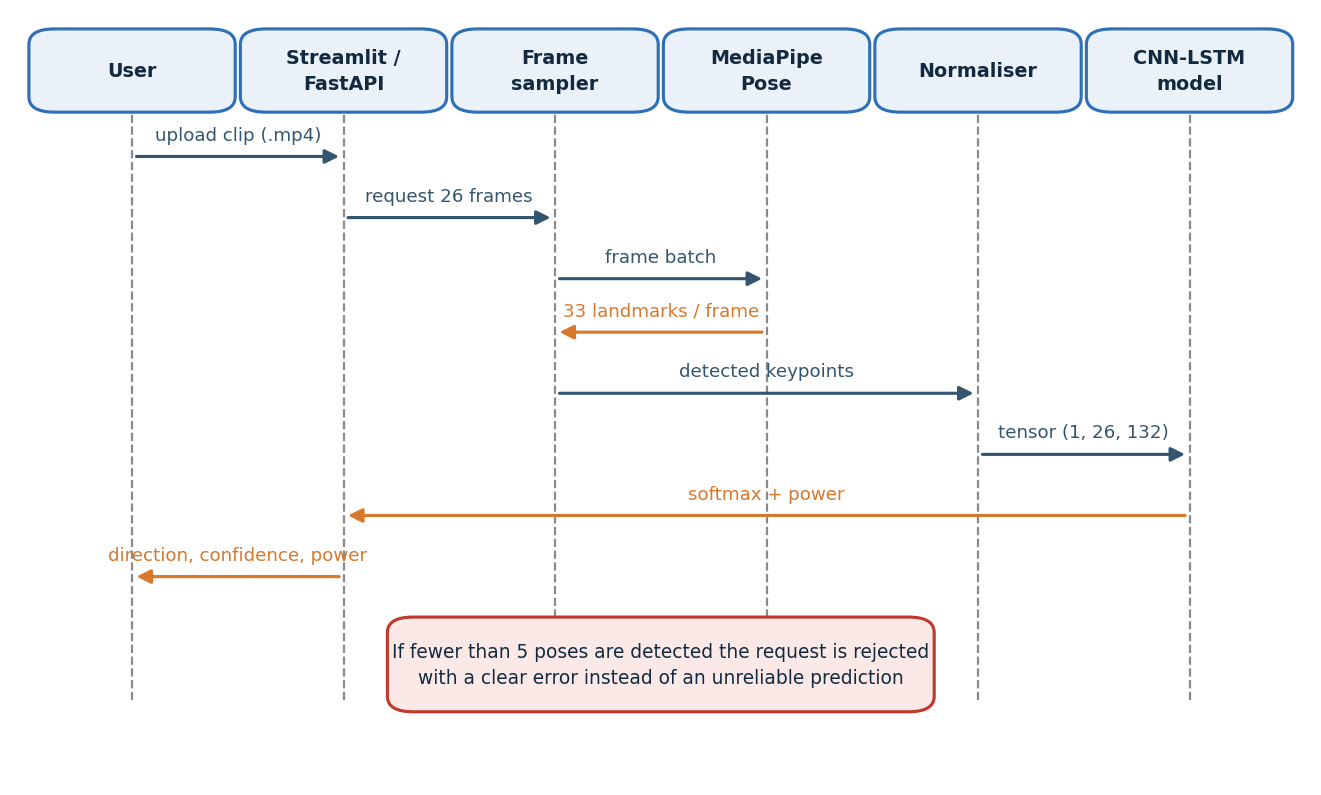
\includegraphics[width=0.99\textwidth]{fig09_inference_sequence.png}
    \caption{Sequence diagram of the inference path for an uploaded clip}
    \label{fig:inference}
\end{figure}

\noindent
\textbf{Description:} This sequence diagram traces a single prediction request. The user uploads a clip, the interface requests a frame sample, MediaPipe returns landmarks for each frame, the normaliser produces a tensor of shape one by twenty six by one hundred and thirty two, and the model returns a softmax distribution together with a power value. The guard shown at the bottom is important: if too few poses are detected the request is refused with an explicit error rather than answered with a prediction derived from an unusable skeleton stream, which mirrors at inference time the quality gate applied during training.

\section{Experiments Conducted}

Two distinct families of experiment are reported in Chapter 4, and it is worth separating them clearly because they answer different questions.

The first family is the development history, comprising five complete training runs whose logs are preserved in \texttt{outputs/model}. These runs differ from one another in the state of the annotation file and in the correctness of the pipeline at the time they were executed, since the corpus grew as locally recorded footage was added, a defect in the mirror augmentation was identified and corrected, and a portion of the direction labels was re-verified against the footage. These runs therefore document how the result improved as the data and the code improved, and the highest validation direction accuracy observed anywhere in the project, 55.9 percent at epoch twenty nine, comes from this family.

The second family is the controlled ablation study, comprising six configurations trained under identical conditions with a fixed seed on the current data, differing from the full model by exactly one factor each. These runs answer the question of which design decisions actually contribute, and because they share a seed and a split they support attribution in a way the development history cannot. The reference model used for every test set number and every evaluation figure in Chapter 4 is the full configuration from this second family, so that the confusion matrix, the per class metrics and the power regression plots all describe one single reproducible checkpoint rather than a mixture of runs.

\clearpage
